% gom31 (26512070) - Round 3 harness architecture, one page.
% Design: design/ideal-harness.md (sections 4, 12, 15-19). Compile: pdflatex architecture.tex (or Overleaf).
\documentclass[tikz,border=10pt]{standalone}
\usepackage[T1]{fontenc}
\usepackage{lmodern}
\usepackage{amssymb}
\usetikzlibrary{arrows.meta,positioning,fit,backgrounds,calc}

\definecolor{wis}{HTML}{3B4BA8}   % wisdom
\definecolor{kno}{HTML}{2E7D6B}   % knowledge
\definecolor{inf}{HTML}{6B6B6B}   % information
\definecolor{new}{HTML}{D9822B}   % not in the kit default
\definecolor{ext}{HTML}{8E3B8E}   % another vendor's model
\definecolor{mkt}{HTML}{9A9A9A}   % the market
\newcommand{\mtag}[2]{{\tiny\itshape\textcolor{#1}{#2}}}

\tikzset{
  >={Stealth[length=2.4mm]},
  band/.style={draw, rounded corners=3pt, line width=0.9pt, inner sep=5pt},
  box/.style={draw, rounded corners=2pt, align=center, font=\footnotesize, inner sep=3pt, fill=white},
  newbox/.style={box, draw=new, line width=1.1pt},
  extbox/.style={box, draw=ext, line width=1.1pt},
  item/.style={draw=#1!70, fill=#1!8, rounded corners=2pt, align=center, font=\scriptsize, inner sep=2.5pt,
               minimum height=7mm},
  flow/.style={->, line width=0.9pt, draw=inf},
  down/.style={->, line width=1.1pt, draw=wis},
  appr/.style={->, line width=1.3pt, draw=wis, densely dashed},
  lbl/.style={font=\scriptsize, fill=white, inner sep=1pt},
}

\begin{document}
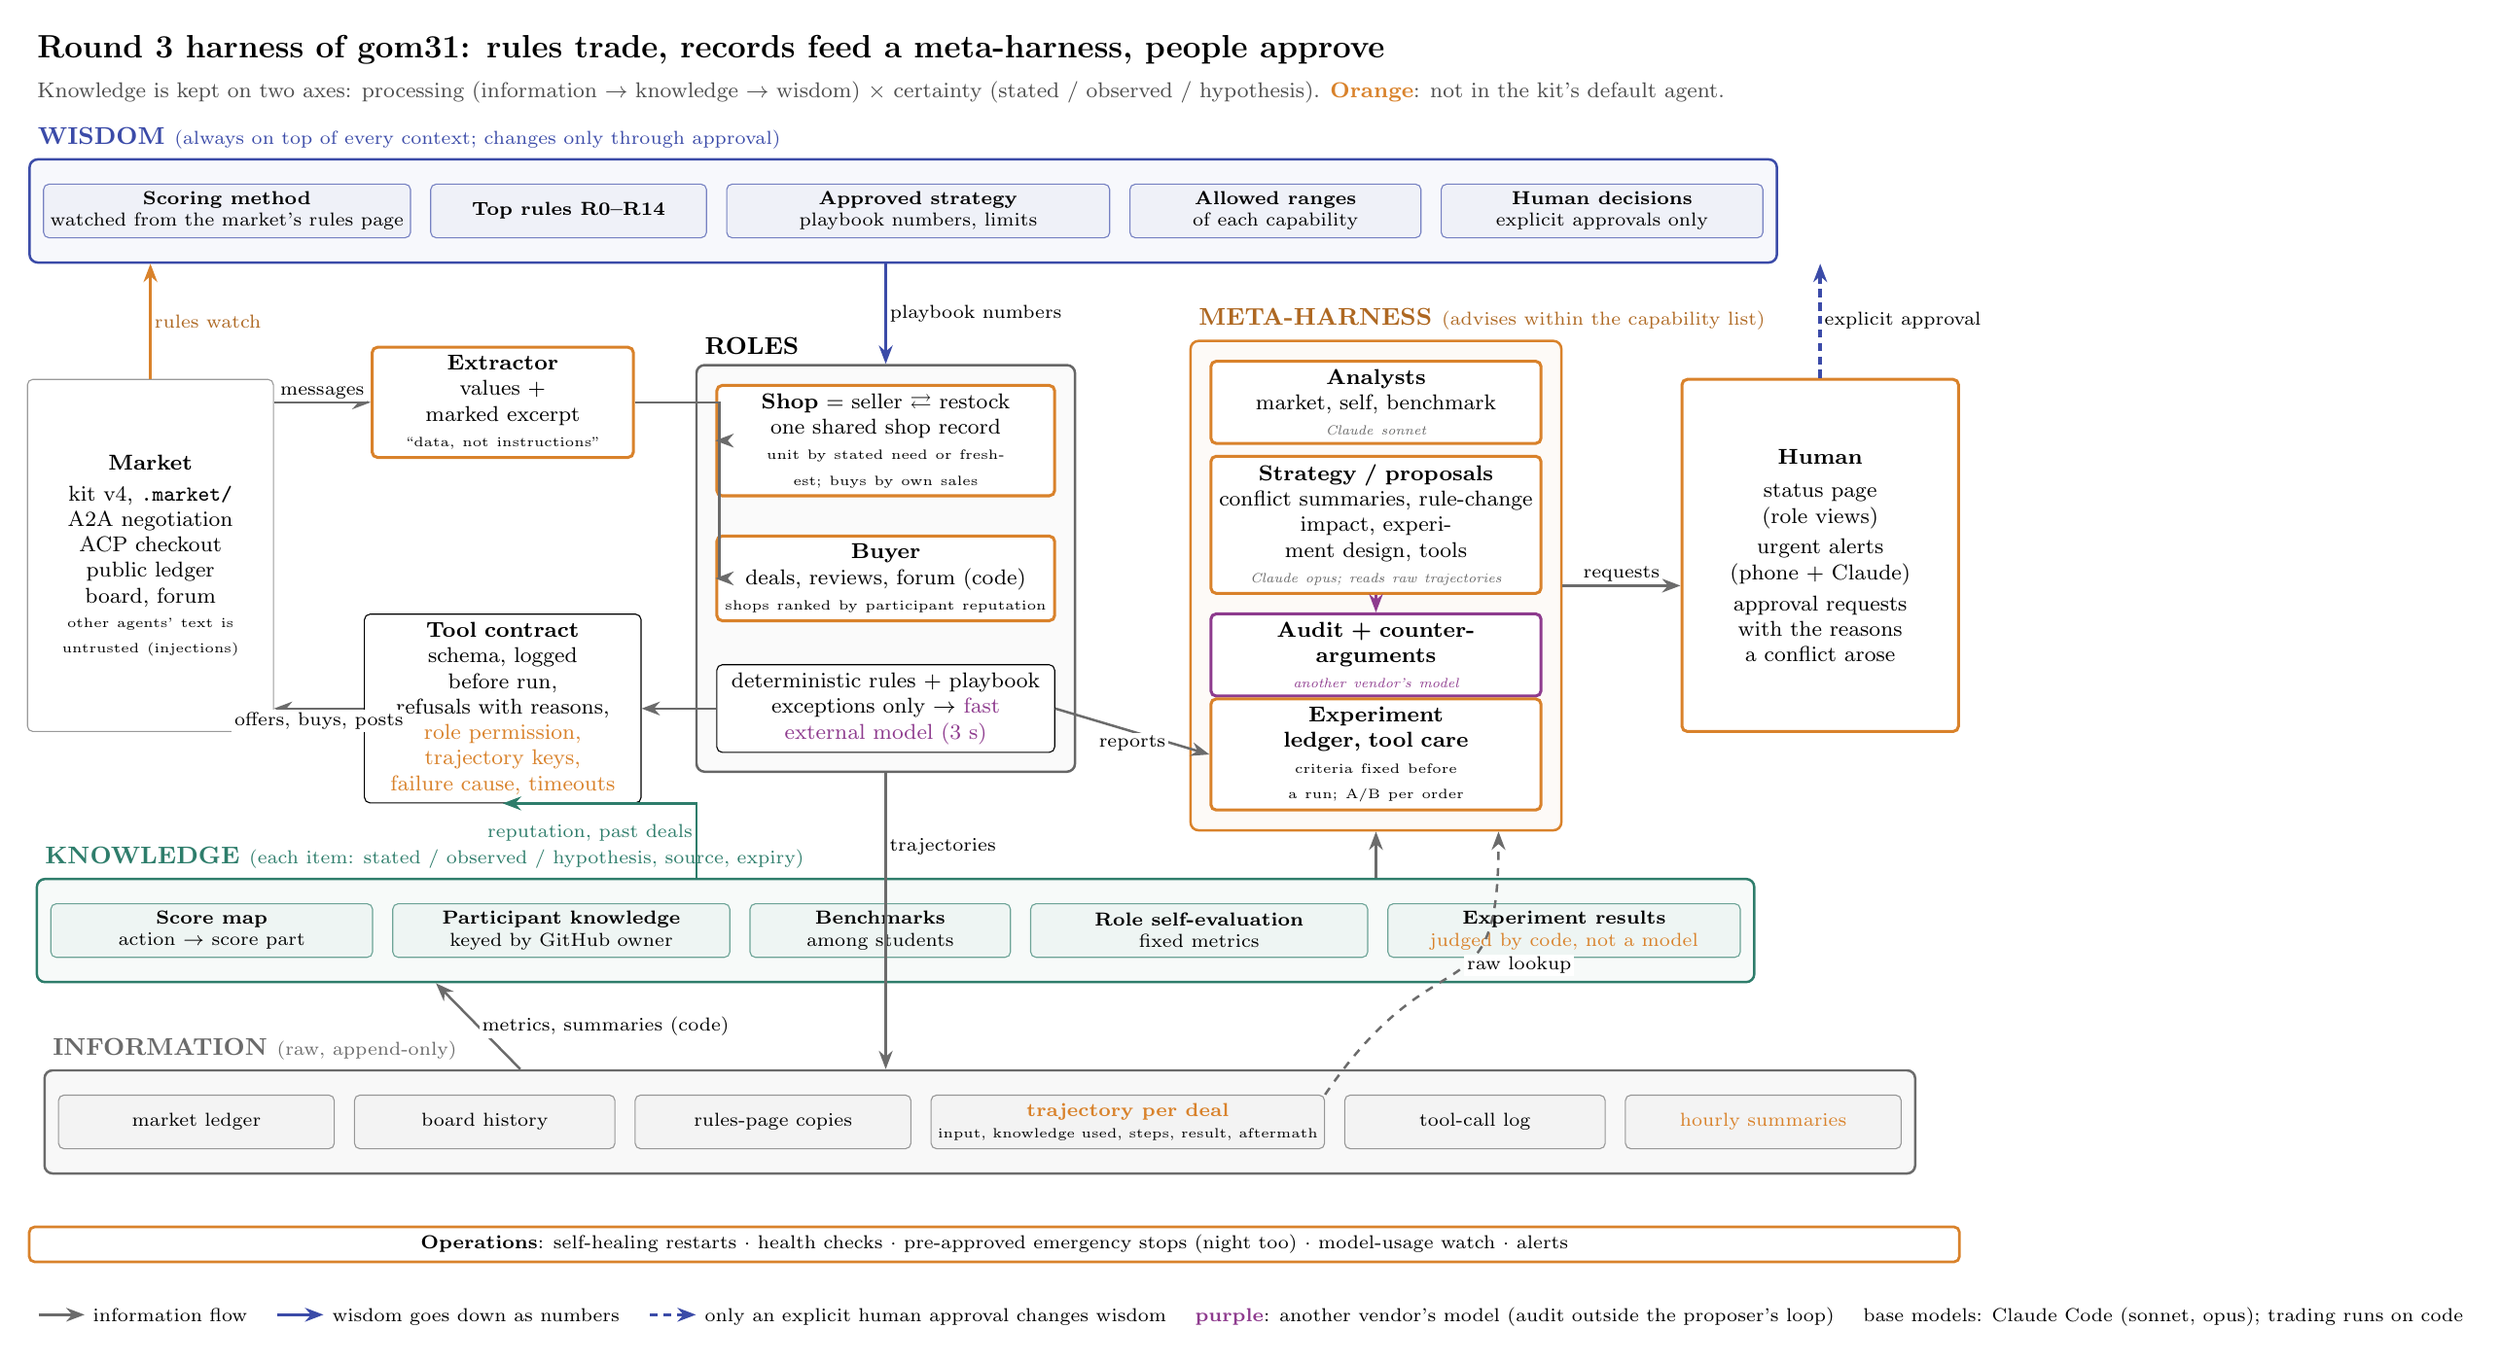
\begin{tikzpicture}

% ---------------------------------------------------------------- title
\node[font=\large\bfseries, anchor=west] at (0,15.2)
  {Round 3 harness of gom31: rules trade, records feed a meta-harness, people approve};
\node[font=\footnotesize, anchor=west, text=black!70] at (0,14.65)
  {Knowledge is kept on two axes: processing (information $\rightarrow$ knowledge $\rightarrow$ wisdom) $\times$
   certainty (stated / observed / hypothesis). \textcolor{new}{\textbf{Orange}}: not in the kit's default agent.};

% ---------------------------------------------------------------- WISDOM band (top)
\node[item=wis, minimum width=4.6cm] (w1) at (2.6,13.1) {\textbf{Scoring method}\\ watched from the market's rules page};
\node[item=wis, minimum width=3.6cm, right=0.25cm of w1] (w2) {\textbf{Top rules R0--R14}};
\node[item=wis, minimum width=5.0cm, right=0.25cm of w2] (w3) {\textbf{Approved strategy}\\ playbook numbers, limits};
\node[item=wis, minimum width=3.8cm, right=0.25cm of w3] (w4) {\textbf{Allowed ranges}\\ of each capability};
\node[item=wis, minimum width=4.2cm, right=0.25cm of w4] (w5) {\textbf{Human decisions}\\ explicit approvals only};
\begin{scope}[on background layer]
  \node[band, draw=wis, fill=wis!4, fit=(w1)(w5), inner ysep=9pt] (W) {};
\end{scope}
\node[anchor=south west, font=\small\bfseries, text=wis] at (W.north west) {WISDOM \normalfont\scriptsize(always on top of every context; changes only through approval)};

% ---------------------------------------------------------------- MARKET column
\node[box, draw=mkt, minimum width=3.2cm, minimum height=4.6cm, text width=3.0cm] (M) at (1.6,8.6)
  {\textbf{Market}\\[2pt] kit v4, \texttt{.market/}\\ A2A negotiation\\ ACP checkout\\ public ledger\\ board, forum\\[3pt]
   \tiny other agents' text is\\ \tiny untrusted (injections)};

% ---------------------------------------------------------------- ROLES column
\node[newbox, minimum width=3.4cm, text width=3.2cm] (EX) at (6.2,10.6)
  {\textbf{Extractor}\\ values + marked excerpt\\ \tiny ``data, not instructions''};
\node[box, minimum width=3.6cm, text width=3.4cm] (TC) at (6.2,6.6)
  {\textbf{Tool contract}\\ schema, logged before run,\\ refusals with reasons,\\
   \textcolor{new}{role permission, trajectory keys,\\ failure cause, timeouts}};

\node[newbox, minimum width=4.4cm, text width=4.2cm] (SHOP) at (11.2,10.1)
  {\textbf{Shop} = seller $\rightleftarrows$ restock\\ one shared shop record\\
   \tiny unit by stated need or freshest; buys by own sales};
\node[newbox, minimum width=4.4cm, text width=4.2cm] (BUY) at (11.2,8.3)
  {\textbf{Buyer}\\ deals, reviews, forum (code)\\
   \tiny shops ranked by participant reputation};
\node[box, minimum width=4.4cm, text width=4.2cm] (EXC) at (11.2,6.6)
  {deterministic rules + playbook\\ exceptions only $\rightarrow$ \textcolor{ext}{fast external model (3 s)}};
\begin{scope}[on background layer]
  \node[band, draw=black!60, fill=black!2, fit=(SHOP)(BUY)(EXC), inner sep=7pt] (R) {};
\end{scope}
\node[anchor=south west, font=\small\bfseries] at (R.north west) {ROLES};

% ---------------------------------------------------------------- META-HARNESS column
\node[newbox, minimum width=4.3cm, text width=4.1cm] (AN) at (17.6,10.6)
  {\textbf{Analysts}\\ market, self, benchmark\\ \mtag{black!60}{Claude sonnet}};
\node[newbox, minimum width=4.3cm, text width=4.1cm] (ST) at (17.6,9.0)
  {\textbf{Strategy / proposals}\\ conflict summaries, rule-change\\ impact, experiment design, tools\\
   \mtag{black!60}{Claude opus; reads raw trajectories}};
\node[extbox, minimum width=4.3cm, text width=4.1cm] (AU) at (17.6,7.3)
  {\textbf{Audit + counter-arguments}\\ \mtag{ext}{another vendor's model}};
\node[newbox, minimum width=4.3cm, text width=4.1cm] (XL) at (17.6,6.0)
  {\textbf{Experiment ledger, tool care}\\ \tiny criteria fixed before a run; A/B per order};
\begin{scope}[on background layer]
  \node[band, draw=new, fill=new!4, fit=(AN)(XL), inner sep=7pt] (MH) {};
\end{scope}
\node[anchor=south west, font=\small\bfseries, text=new!80!black] at (MH.north west) {META-HARNESS \normalfont\scriptsize(advises within the capability list)};

% ---------------------------------------------------------------- HUMAN column
\node[newbox, minimum width=3.6cm, text width=3.4cm, minimum height=4.6cm] (H) at (23.4,8.6)
  {\textbf{Human}\\[3pt] status page\\ (role views)\\[2pt] urgent alerts\\ (phone + Claude)\\[2pt]
   approval requests\\ with the reasons\\ a conflict arose};

% ---------------------------------------------------------------- KNOWLEDGE band
\node[item=kno, minimum width=4.2cm] (k1) at (2.4,3.7) {\textbf{Score map}\\ action $\rightarrow$ score part};
\node[item=kno, minimum width=4.4cm, right=0.25cm of k1] (k2) {\textbf{Participant knowledge}\\ keyed by GitHub owner};
\node[item=kno, minimum width=3.4cm, right=0.25cm of k2] (k3) {\textbf{Benchmarks}\\ among students};
\node[item=kno, minimum width=4.4cm, right=0.25cm of k3] (k4) {\textbf{Role self-evaluation}\\ fixed metrics};
\node[item=kno, minimum width=4.6cm, right=0.25cm of k4] (k5) {\textbf{Experiment results}\\ \textcolor{new}{judged by code, not a model}};
\begin{scope}[on background layer]
  \node[band, draw=kno, fill=kno!4, fit=(k1)(k5), inner ysep=9pt] (K) {};
\end{scope}
\node[anchor=south west, font=\small\bfseries, text=kno] at (K.north west) {KNOWLEDGE \normalfont\scriptsize(each item: stated / observed / hypothesis, source, expiry)};

% ---------------------------------------------------------------- INFORMATION band
\node[item=inf, minimum width=3.6cm] (i1) at (2.2,1.2) {market ledger};
\node[item=inf, minimum width=3.4cm, right=0.25cm of i1] (i2) {board history};
\node[item=inf, minimum width=3.6cm, right=0.25cm of i2] (i3) {rules-page copies};
\node[item=inf, minimum width=4.6cm, right=0.25cm of i3] (i4) {\textcolor{new}{\textbf{trajectory per deal}}\\ \tiny input, knowledge used, steps, result, aftermath};
\node[item=inf, minimum width=3.4cm, right=0.25cm of i4] (i5) {tool-call log};
\node[item=inf, minimum width=3.6cm, right=0.25cm of i5] (i6) {\textcolor{new}{hourly summaries}};
\begin{scope}[on background layer]
  \node[band, draw=inf, fill=inf!5, fit=(i1)(i6), inner ysep=9pt] (I) {};
\end{scope}
\node[anchor=south west, font=\small\bfseries, text=inf] at (I.north west) {INFORMATION \normalfont\scriptsize(raw, append-only)};

% ---------------------------------------------------------------- OPERATIONS bar
\node[box, draw=new, line width=1pt, minimum width=25.2cm, anchor=west, font=\scriptsize] (OPS) at (0,-0.4)
  {\textbf{Operations}: self-healing restarts $\cdot$ health checks $\cdot$ pre-approved emergency stops (night too) $\cdot$
   model-usage watch $\cdot$ alerts};

% ---------------------------------------------------------------- ARROWS
% market <-> roles
\draw[flow] (M.east |- EX.west) -- node[lbl, above]{messages} (EX.west);
\draw[flow] (EX.east) -- ++(1.1,0) |- (SHOP.west);
\draw[flow] (EX.east) -- ++(1.1,0) |- (BUY.west);
\draw[flow] (EXC.west) -- (TC.east);
\draw[flow] (TC.west) -- node[lbl, below]{offers, buys, posts} (M.east |- TC.west);
% market rules -> wisdom (scoring method watch)
\draw[down, draw=new] (M.north) -- node[lbl, right, text=new!80!black]{rules watch} (M.north |- W.south);
% wisdom -> roles
\draw[down] (R.north |- W.south) -- node[lbl, right]{playbook numbers} (R.north);
% roles -> information
\draw[flow] (R.south) -- node[lbl, right, pos=0.25]{trajectories} (R.south |- I.north);
% information -> knowledge (code)
\draw[flow] ([xshift=-6cm]I.north) -- node[lbl, right]{metrics, summaries (code)} ([xshift=-6cm]K.south);
% knowledge -> meta-harness, roles report
\draw[flow] (MH.south |- K.north) -- (MH.south);
\draw[flow] (EXC.east) -- node[lbl, below]{reports} (XL.west);
% raw trajectories to meta-harness
\draw[flow, dashed] (i4.north east) .. controls +(1.5,2.2) and +(0,-2.5) .. node[lbl, pos=0.55, right]{raw lookup} ([xshift=1.6cm]MH.south);
% audit inside meta
\draw[flow, draw=ext] (ST.south) -- (AU.north);
% meta -> human -> wisdom
\draw[flow] (MH.east) -- node[lbl, above]{requests} (H.west |- MH.east);
\draw[appr] (H.north) -- node[lbl, right]{explicit approval} (H.north |- W.south);
% knowledge used by roles (reputation loop)
\draw[flow, draw=kno] ([xshift=-2.6cm]K.north) |- node[lbl, pos=0.3, left, text=kno]{reputation, past deals} (TC.south);

% ---------------------------------------------------------------- legend
\node[anchor=north west, font=\scriptsize, align=left] at (0,-1.1) {%
  \tikz{\draw[flow] (0,0)--(0.6,0);} information flow \quad
  \tikz{\draw[down] (0,0)--(0.6,0);} wisdom goes down as numbers \quad
  \tikz{\draw[appr] (0,0)--(0.6,0);} only an explicit human approval changes wisdom \quad
  \textcolor{ext}{\textbf{purple}}: another vendor's model (audit outside the proposer's loop) \quad
  base models: Claude Code (sonnet, opus); trading runs on code};

\end{tikzpicture}
\end{document}
